\chapter{Organization of the Project Team}
\label{cha:projektteam-arbeiten}

The WASA2 (Web Applications and Service-oriented Architectures 2) is a lecture for master students
offered by C\&M each summer semester. The lecture is accompanied by a mandatory practical course.
The goal of the practical course is to deepen the understanding of the concepts discussed in the WASA2
lecture. The practical course is described in Section \ref{sec:wasa2_overview}.
The author of this thesis supervised a team participating in the practical course.
The contributions of the author to the practical course and the work of the project team are described in Section \ref{sec:p3}.

\section{Overview of the WASA2 Lecture and Practical Course}
\label{sec:wasa2_overview}

\begin{figure}[tb]
	\centering
	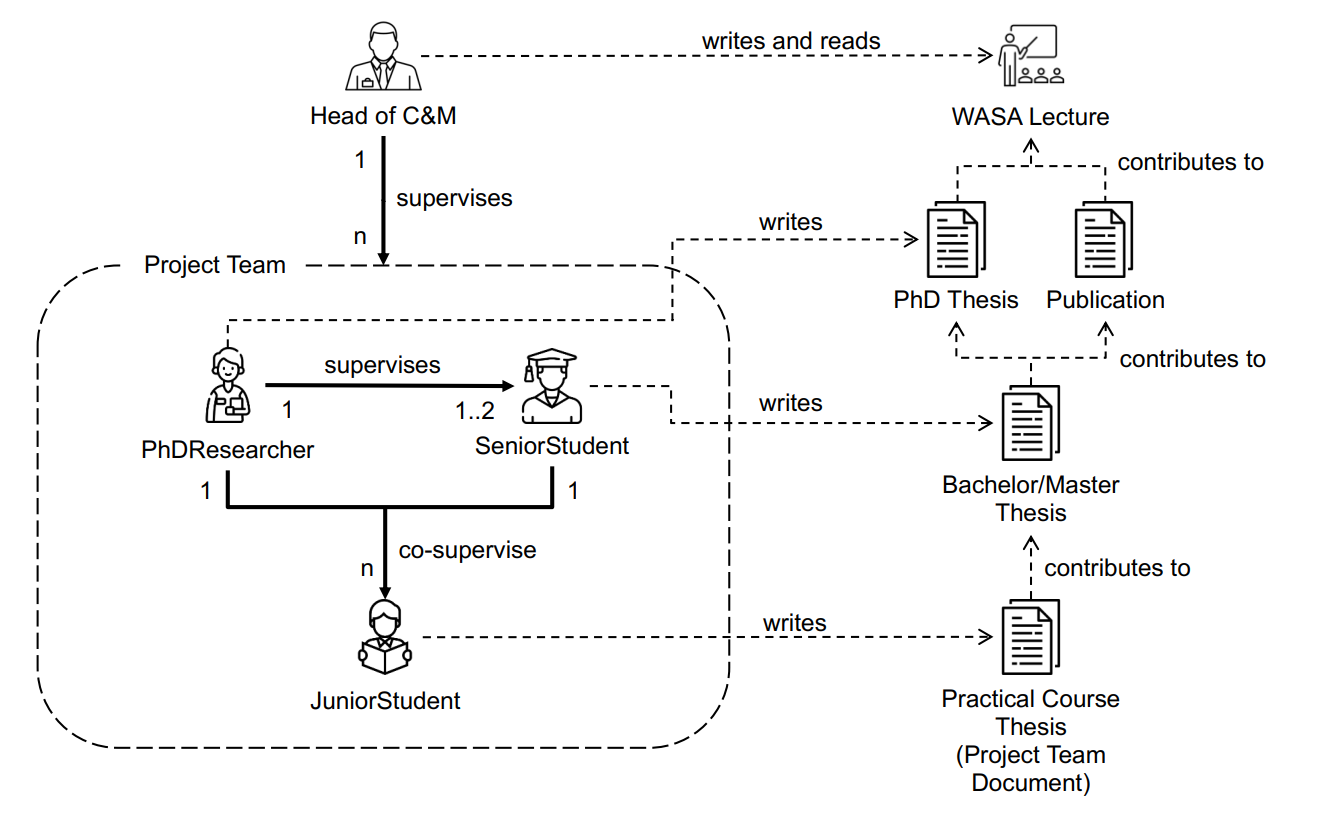
\includegraphics[width=0.7\textwidth]{figures/7.1_practical_course_roles.png}
	\caption{WASA2 Practical Course Supervision Hierarchy \cite{CM-W-INT}}
	\label{fig:practical_course_roles}
\end{figure}

The WASA2 lecture is accompanied by a mandatory practical course.
The participants of the practical course are organized into the teams P1 Microservice Engineering,
P2 Access Management, and P3 DevOps. The team P1 Microservice Engineering focused on contributing
to the BestRentalPoC by implementing the microservice RentalManagement and ensuring its
quality through testing.
P2 Access Management focused on the integration of authorization policies into the demonstrator
project from the winter semester 2022/2023 which was called CCSApp. They also analyzed
different authorization architectures.
P3 DevOps focused on the usage of the DevOps concept to automate the provisioning
of Microsoft Azure cloud resources that are needed by the decentralized identity solution
that BestRentalPoC employs. This team was in part supervised by the author of this thesis.

The practical course has a supervision hierarchy that assigns both the participating students
as well as the members of the C\&M group a role. This hierarchy can be seen in Figure \ref{fig:practical_course_roles}.
The professor holding the lecture holds
the role of Head of C\&M and is ultimately responsible for supervising the course.
The Head of C\&M creates the WASA2 lecture.
Each project team is supervised by one PhDResearcher and one or more SeniorStudents.
The PhDResearcher is a member of the C\&M group who is currently working on their PhD thesis and is supervised by the Head of C\&M.
The PhDResearchers contribute directly to the WASA2 lecture through their PhD thesis and their publications.
SeniorStudents are students who are currently writing their bachelor's or master's thesis
at the C\&M group and are supervised by the PhDResearchers. They contribute to the PhD thesis' and the publications of the PhDResearchers
through work on their thesis'.
The students who are participating in the practical course have the role
of JuniorStudent. Each JuniorStudent writes a practical course thesis throughout their participation in the course
which provides the main basis for their final grade. 
Their practical course thesis contributes to the thesis' of the SeniorStudents.
In addition to their practical course thesis, the JuniorStudents also create
a project team presentation in which they present their team's work to their fellow JuniorStudents.
This project team presentation takes place during the WASA2 lecture.

The practical course is split into three phases familiarization, supervised work,
and unsupervised work. The first phase, familiarization, spans the first two weeks of the practical
course. During this phase, the JuniorStudents focus on familiarizing themselves with the working
processes of the C\&M group which are documented in the C\&M teamwork document \cite{CM-W-TEA}.
They also familiarize themselves with the demonstrator project of the semester by describing
its current state in their practical course thesis. During the second phase, supervised work,
the JuniorStudents work in close collaboration with their SeniorStudents and their PhDResearcher
to create the basis for their team's project. This basis is then used
by the JuniorStudents in the third phase, unsupervised work, to complete their team's project
without any major assistance from their supervisors.

To ensure that the JuniorStudents met the expectation of how many hours of work
the practical course requires as set forth by the ECTS (The European Credit Transfer and Accumulation System)
points gained by the practical course, the JuniorStudents have to keep a time sheet.
The practical course grants 5 ECTS points which each require 30 hours of work, totalling 150 hours of work.

The teams of the practical course meet in a weekly meeting to discuss their practical course
thesis as well as the status of their tasks. Prior to the weekly meetings, the JuniorStudents
provide a current version of their practical course thesis that is ready to be reviewed
by their supervising SeniorStudents. The SeniorStudents review these documents and provide
feedback which is discussed in the following weekly team meeting. Along with the document,
the JuniorStudents send a weekly status update email to their SeniorStudents and PhDResearcher
to signal them that all of their documents are in order and ready to be reviewed.

\section{Project Team P3 DevOps}
\label{sec:p3}

The author of this thesis supervised the project team P3 DevOps that participated in the
WASA2 practical course. Team P3 focused on the provisioning of resources for the BestRentalPoC.
The three phases of the practical course were planned as follows.
During the first phase of familiarization, the JuniorStudents would learn about the required
technologies for provisioning BestRentalPoC and create a concept for its provisioning.
The second phase would focus on creating a sample demonstration implementation
of the provisioning concept from the previous phase and validating it.
The final phase would then see the validated provisioning concept be applied to BestRentalPoC.

The JuniorStudents of team P3 DevOps started the practical course by writing a description
of BestRentalPoC in its current state for their practical course thesis. They also started
to read the documentation of Entra (Microsoft Entra Verified Id) which is the decentralized identity
solution used by BestRentalPoC. In the next step, the students then had to provision
a GitLab repository using Crossplane. Crossplane is the tool that was later used to provision
resources in Microsoft Azure. After this, the team was split into two groups.
The first group focused on the provisioning tasks for the BestRentalPoC and was therefore called Provisioning.
This group was supervised by a student working on his master's thesis. A description
of the Provisioning group's tasks and their results can be found in his master's thesis \cite{Go23}.
The second group, called Monitoring, focused on assisting the author of this thesis with integrating SPMonitor into the BestRentalPoC.

\begin{figure}[tb]
	\centering
	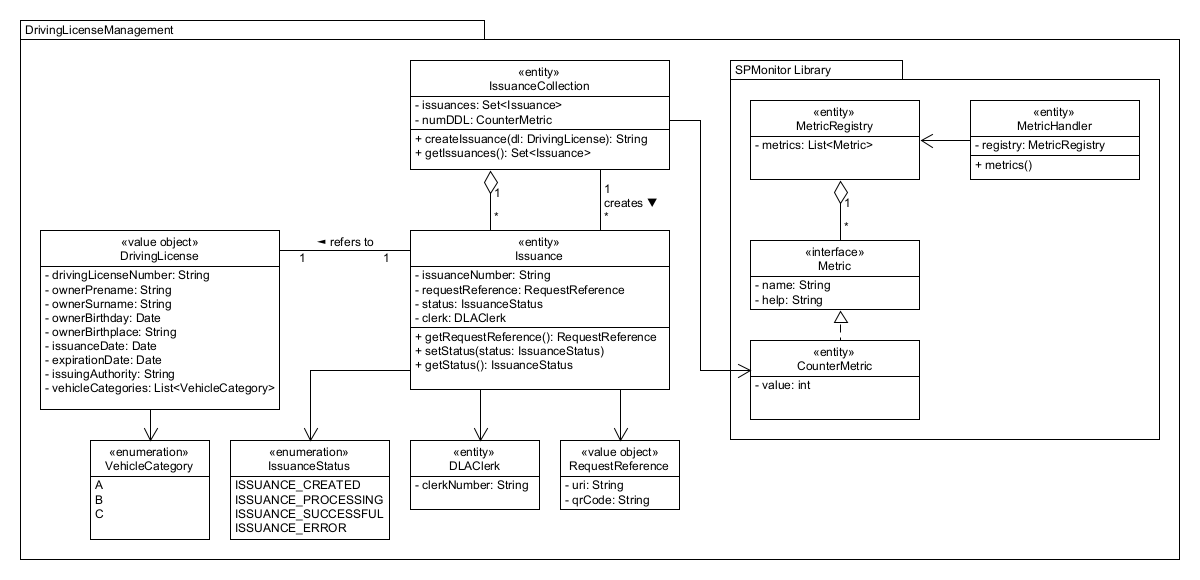
\includegraphics[width=\textwidth]{figures/7.2_api_diagram_drivinglicensemanagement.png}
	\caption{API Diagram Application Microservice DrivingLicenseManagement}
	\label{fig:api_diagram_drivinglicensemanagement_p3}
\end{figure}

The Monitoring group started their work by familiarizing themselves with this thesis as well as with the work
of project team P1 Microservice Engineering who were responsible for creating the microservice
AM-DrivingLicenseManagement (Application Microservice DrivingLicenseManagement) for the BestRentalPoC.
The next task of the Monitoring group was the adaptation of the API diagram of AM-DrivingLicenseManagement
to include the SPMonitor Library that was developed in Chapter \ref{cha:first_solution}.
The adapted API diagram can be seen in Figure \ref{fig:api_diagram_drivinglicensemanagement_p3}.
The adaptation consists of creating a representation of the SPMonitor Library in the API diagram
and adding a CounterMetric called numDDL to the IssuanceCollection entity.

After this, the second phase of supervised work started. 
The Monitoring group started this phase by creating a PoC (Proof of Concept)
implementation of the SPMonitor Library. During the development of the second phase, the project team also
had to plan and create a project team presentation. The project team presentation is presented during the WASA2 lecture
where each project team presents their work to the other teams. The team P3 worked on this in parallel to their other tasks.
After the PoC implementation of SPMonitor Library had been created and reviewed by the author of this thesis, it was decided
that the PoC implementation was ready to be integrated into the microservice AM-DrivingLicenseManagement.
In preparation for the integration into the microservice AM-DrivingLicenseManagement, the SPMonitor Library was turned into
a standalone Golang module that could be used by AM-DrivingLicenseManagement as a dependency.
The project team P1 had already implemented the microservice AM-DrivingLicenseManagement at this point.
This meant that the SPMonitor Library could be added to the list of dependencies of AM-DrivingLicenseManagement
and then integrated into the microservice. The integration of SPMonitor library into AM-DrivingLicenseManagement
consisted of adding a new endpoint to the microservice under the path /metrics through which the metrics of AM-DrivingLicenseManagement
could be collected. Additionally, a CounterMetric was created in the microservice which would increment the value of the numDDL metric
every time that a digital driving license was successfully issued by the microservice. This can be seen in Listing \ref{lis:am_dlm_num_ddl}.
The variable numDDLMetric is a CounterMetric and was created during the creation of the IssuanceOperations.
After the issuance flow for a digital driving license is completed either because it succeeded or failed,
AM-DrivingLicenseManagement receives a request to its so-called callback endpoint which is used by Microsoft Entra Verified Id \cite{MIC-ENT}
to signal the completion of the issuance flow. The request to the callback endpoint contains a request status
that can either be IssuanceCreated, IssuanceProcessing, IssuanceSuccessful, or IssuanceError.
During the handling of the callback request, the function shown in Listing \ref{lis:am_dlm_num_ddl} is called.
If the request status of the issuance is IssuanceSuccessful in line 3, the numDDL metric is incremented in line 4.

After the SPMonitor Library was integrated into AM-DrivingLicenseManagement,
the groups of the project team P3 combined into one group again for the third phase of unsupervised work
and solely focused on the provisioning of resources for BestRentalPoC.
The author of this thesis did not supervise this part of the practical
course except for reviews and feedback for the practical course thesis' of the team. The remaining
tasks, as well as the tasks of the Provisioning group, can be read in the master's thesis of the student
who supervised this part of the practical course \cite{Go23}.

\begin{lstlisting}[caption = {Usage of the SPMonitor Library in AM-DrivingLicenseManagement}, label = {lis:am_dlm_num_ddl}, style = kit-cm, language=Go]
func (ops *IssuanceOperations) SetStatus(requestStatus string) {
	ops.issuance.Status = mappers.MapIssuanceStatus(requestStatus)
	if ops.issuance.Status == model.IssuanceSuccessful {
		ops.numDDLMetric.Increment()
	}
	// ...
}
\end{lstlisting}